\chapter{Introduction}

In this thesis, we deal with parallelization of speeding up cluster analysis and dependency between input data properties and different approaches to parallelization.
The main motivation for choosing this topic was not very widespread use of graphics cards whose performance with each generation increases rapidly. We want to use this potential to accelerate the current algorithmic problems, which are very compute-intensive. Such problems include the right cluster analysis, which has a very broad scope of application so it is very useful to accelerate it using the most modern hardware.

\section{Cluster Analysis} \label{sec:clusteranalysis}
Cluster analysis is a task that assigns a group to each object from the input set so that each group consists of objects with similar properties. Similar means that same property of two objects differs minimally in comparsion to same property of other objects. This means that each cluster contains objects that are more similar than objects from other groups. Hence the cluster analysis may be performed only on sets of objects of which must each be described by the same set of properties. This analysis has a wide range of applications, such as data mining, pattern recognition, machine learning, and many more.\\
Cluster analysis itself is only a task to be solved, not a concrete algorithm. There are many ways to solve this task, but they differ significantly in defining what cluster is and in cluster search efficiency. Most commonly definitions of the cluster are groups with small distances between the objects from the same cluster, dense areas of the input data, intervals or particular statistical distribution.\\
There are also two types of cluster organization. One way is hierarchically ordered clusters creates which creates a system of subsets where the intersection of the two is either the empty set or just one of them or non-hierarchical clusters, which creates system where clusters are disjoint sets. Because of complexity of the hierarchical clustering, in this thesis we deal with non-hierarchical type only.

\section{Cluster Models and Algorithms} \label{sec:clustermodels}
There are so many cluster models and one of the reasons why there exists a large amount of them is that the ``cluster'' cannot be precisely defined~\cite{EstivillCastro02}. Second reason is really wide applicability of this task so people from different departments approach this problem differently, because their notion of cluster differs significantly. \\

There exist many clustering algorithms because of many cluster models but there exist no universal algorithm, such an algorithm that covers all cluster models. Each algorithm was designed to cover one model or a subset of models and usually it is weak or not applicable for other models.\\
Because all of these algorithms counts distance, appropriate metric must be used. Some commonly used metric are:
\begin{description}
\item[Manhattan distance $L_1$] $$\|a-b\|_1=\sum_i |a_i - b_i| $$
\item[Euclidian distance $L_2$] $$\|a-b\|_2=\sqrt{\sum_i (a_i - b_i)^2 }$$
\item[Squared Euclidian distance $L_2^2$] $$\|a-b\|_2^2=\sum_i (a_i - b_i)^2 $$
\item[$p$-norm distance $L_p$] $$\|a-b\|_p=(\sum_i |a_i - b_i|^p)^\frac{1}{p} $$
\item[Maximum distance $L_\infty$] $$\|a-b\|_\infty=\lim_{p\to\infty}(\sum_i |a_i - b_i|^p)^\frac{1}{p}=\max_i |a_i - b_i| $$
\end{description}
All of these methods are only applicable for numeric data, so for other types, different metrics must be used (for example, Levenshtein for text, Mahalanobis for distance between point and distribution).
\\
The most typical models of clusters and algorithms are:
\begin{description}
\item[Well-Separated Clusters] Objects are well separated. Cluster is a set of objects such that each object in cluster is closer to objects from its cluster than to objects from other clusters~\autoref{fig:wellSeparatedObjects}. This is the easiest data input and most of algorithms performs well in this case.

\item[Center-Based Clusters] Object belongs to cluster if it is closer to the ``center'' of the cluster than ``centers'' of all other clusters.~\autoref{fig:centerBasedClusters} Center of cluster is usually called centroid or mean and it could represents whole cluster. This is good model for k-means like algorithms. \\
\textit{\textbf{Center-based clustering}} representing clusters as central object, which may not be part of the input data set.  For example \textit{\textbf{k-means}} algorithm takes $k$ centers and than each object is assigned to nearest center. Again, many metrics could be used, but commonly \textit{Euclidian distance} or \textit{Squared Euclidian distance} is used. \textit{\textbf{k-means}} clustering is basically an optimization problem where we looking for $k$ centers so distances will be the lowest possible. Problem is that optimization itself is NP-hard problem, so solution is commonly only approximate solution is searched. Approximation is commonly done by many iterations consist of assigning clusters to objects and  counting new means.
There are many variants of \textit{\textbf{k-means}} algorithm, they will be described later %TODO add ref too kmeans section
%\begin{description}
%\item[k-medoids] - centers are only objects from input data set
%\item[k-medians] - median is used instead of mean
%\item[k-means++] - initial centers are chosen randomly
%\item[Fuzzy k-means] - fuzzy cluster assignment is allowed
%\end{description}

One of the biggest problems of \textbf{k-means} algorithms is that the number of clusters must be specified at the beginning. Second problem is that clusters with similar size are used (in term of distance, not number of contained objects). This usually leads to splitting bigger clusters into smaller ones, because algorithm optimize cluster centers, not borders.
Output of \textit{\textbf{k-means}} like algorithms is usually input data set split in \textit{Voronoi cells}which could be useful for some problems.

\item[Contiguous Clusters] This model is similar to Center-Based Clusters model but there is difference that two clusters can merge into one. In other words, object is in cluster if it is similar to one ore more other objects from cluster.~\autoref{fig:contiguousClusters}\\
Main idea of \textbf{Contiguity-based clustering} is that objects that are nearby are more related than objects that are farther, so these algorithms grouping objects based on their distance only. Each cluster can be described by sum of distances or by maximum distance needed to connect objects in cluster. Having these cluster property, they can be easily ordered into hierarchy so parent clusters needs little more distance to connect its objects. This hierarchy could be represented as a dendrogram, which is tree diagram showing cluster hierarchy.\\

Other problem is the selection of linkage criterion, because cluster consists of many objects, there are many choices to compute the distance to. There are several methods for choosing linkage criteria between two sets of objects $A$ and $B$, $d$ is chosen metric:
\begin{description}
\item[Maximum or complete linkage clustering] $$\max\{d(a,b) : a \in A, b \in B\}$$
\item[Minimum or single linkage clustering] $$\min\{d(a,b) : a \in A, b \in B\}$$
\item[Mean or average linkage clustering, or UPGMA] (Unweighted Pair Group Method with Arithmetic Mean) $$\frac{1}{|A||B|}\sum_{a \in A} \sum_{b \in B} d(a,b)$$
\item[Centroid linkage clustering, or UPGMC] (Unweighted Pair-Group Method using Centroids) $$\|c_a - c_b\| \mbox{ where } c_a \mbox{ and } c_b \mbox{ are the centroids of clusters } A \mbox{ and } B$$
\item[Minimum energy clustering] $$\frac{2}{nm}\sum_{i,j=1}^{n,m}\|a_i-b_j\|_2-\frac{1}{n^2}\sum_{i,j=1}^{n}\|a_i-a_j\|_2-\frac{1}{m^2}\sum_{i,j=1}^{m}\|b_{i}-b_{j}\|_{2}$$
\end{description}

These methods are not resistive for extreme objects, which cause generating new clusters or even merging others. These methods has generally $O(n^3)$ complexity so they are slow for large amount of data. There exist optimization for special cases which has only complexity $O(n^2)$. These methods are taken as obsolete.

\item[Density-Based Clusters] Clusters are dense regions of objects. They are separated by low-density regions. This method is useful when some noise is present because the low-density regions will cover them and clusters will not change.~\autoref{fig:densityClusters} \\
Clusters in \textbf{Density-based clustering} are defined as areas with higher density of objects than in the rest of input data. Standalone objects are taken as noise. One of the most popular method is \textit{DBSCAN}. It is similar to contiguity-based clustering, because it connecting points based on the distance, but it only connects points satisfying density criterion. This means that in neighborhood specified by distance must be a minimum number of objects. These objects are called core objects and form the basis of cluster. Than objects which do not satisfy the density criterion but are close enough to at least one point from the cluster are added to cluster too.\\
The advantage of this method is its computational modesty, because it require only linear number of range queries. This method is deterministic so there is no need to tun it in iterations.
Drawback of these methods is the $\epsilon$ density parameter so borders of clusters with smaller density could be interpreted as  noise. Also separating nearby clusters may cause problems to these methods.

\item[Distribution models] Clusters in distribution models are objects that belong to same probability distribution. It is possible that one object belongs to more clusters.\\
In \textbf{Distribution-based clustering}, clusters are defined as objects from the same or similar distribution. This approach basically emulates process of generating the input data and try to reconstruct the lost statistical parameters. Main problem of this typ of clustering is problem known as \textit{overfitting}. This means that more complex model is described by less complex one and the difference between them is marked as deviation or noise. For example 3 points from the neighborhood of parabola vertex will be described by linear function.\\
One of methods used in distribution-based clustering is \textit{Gaussian mixture models} where algorithm iteratively optimizing parameters of fixed number of Gaussian distributions.
Problem is that this method assuming Gaussian distributed data set, but this set may not have even a model.

\item[Conceptual Clusters] Objects in cluster has some properties same or similar, but other properties could differ significantly.~\autoref{fig:conceptualClusters}\\
As algorithm for Conceptual Clusters, we can use algorithm depends on other model properties and less significant properties of objects could be easily omitted.

\item[Graph-Based Models] For example cliques in graphs should represent clusters. Clique is subset of nodes where every two nodes are connected with edge.~\autoref{fig:graphClusters}\\
Because of special demands of this model, special algorithms are needed so we could use graph algorithms, for example Bron-Kerbosch algorithm for finding cliques. %TODO source!
\end{description}

\begin{figure}[h]
\centering
\begin{subfigure}{.5\textwidth}
  \centering
  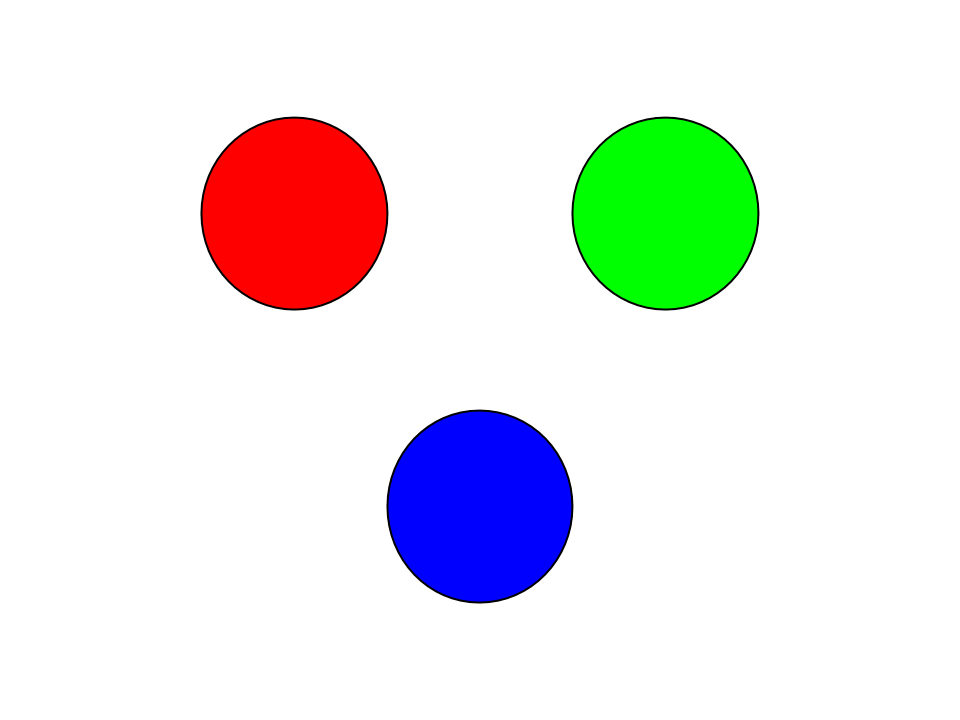
\includegraphics[width=.5\linewidth]{img/wellSeparatedObjects.png}
  \caption{Well sepatated objects}
  \label{fig:wellSeparatedObjects}
\end{subfigure}%
\begin{subfigure}{.5\textwidth}
  \centering
  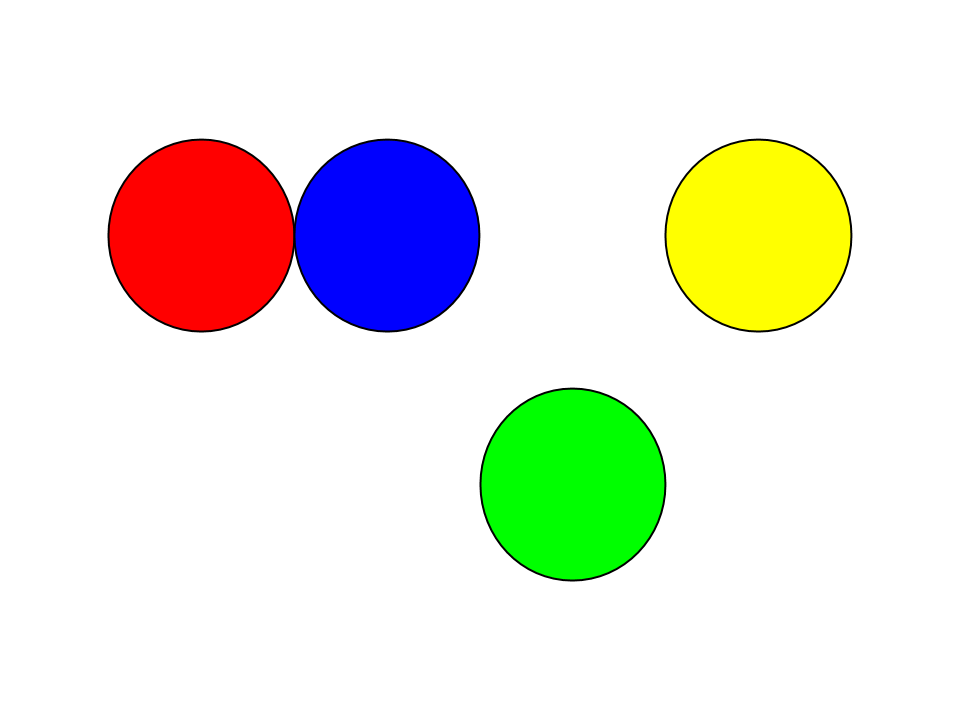
\includegraphics[width=.5\linewidth]{img/centerBasedClusters.png}
  \caption{Center-Based Clusters}
  \label{fig:centerBasedClusters}
\end{subfigure}%
\vspace*{0.5cm} 
\begin{subfigure}{.5\textwidth}
  \centering
  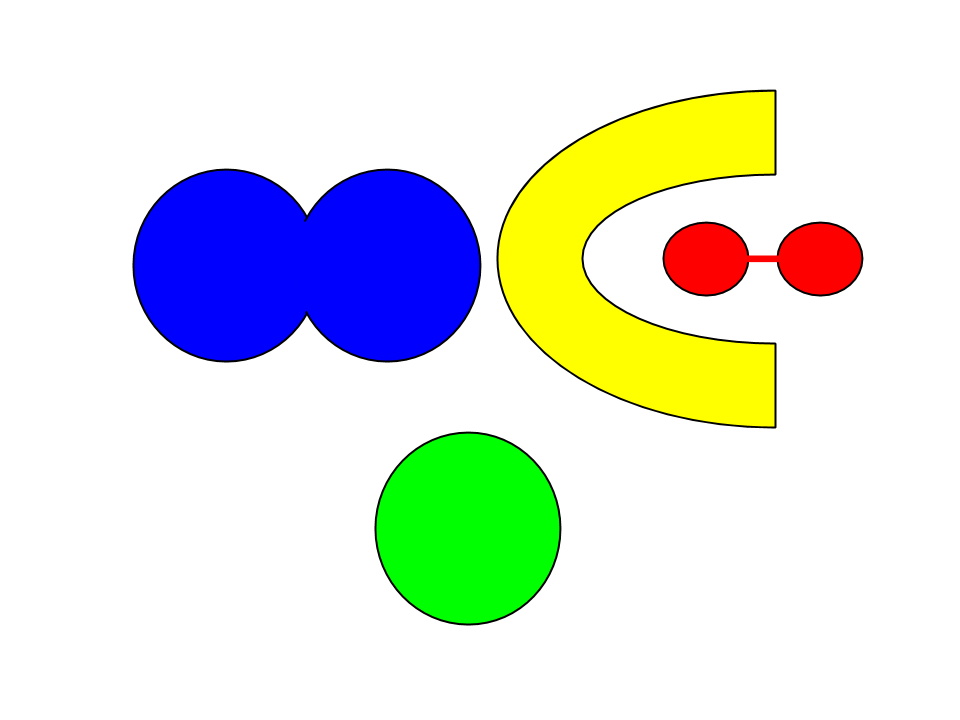
\includegraphics[width=.5\linewidth]{img/contiguousClusters.png}
  \caption{Contiguous Clusters}
  \label{fig:contiguousClusters}
\end{subfigure}%
\begin{subfigure}{.5\textwidth}
  \centering
  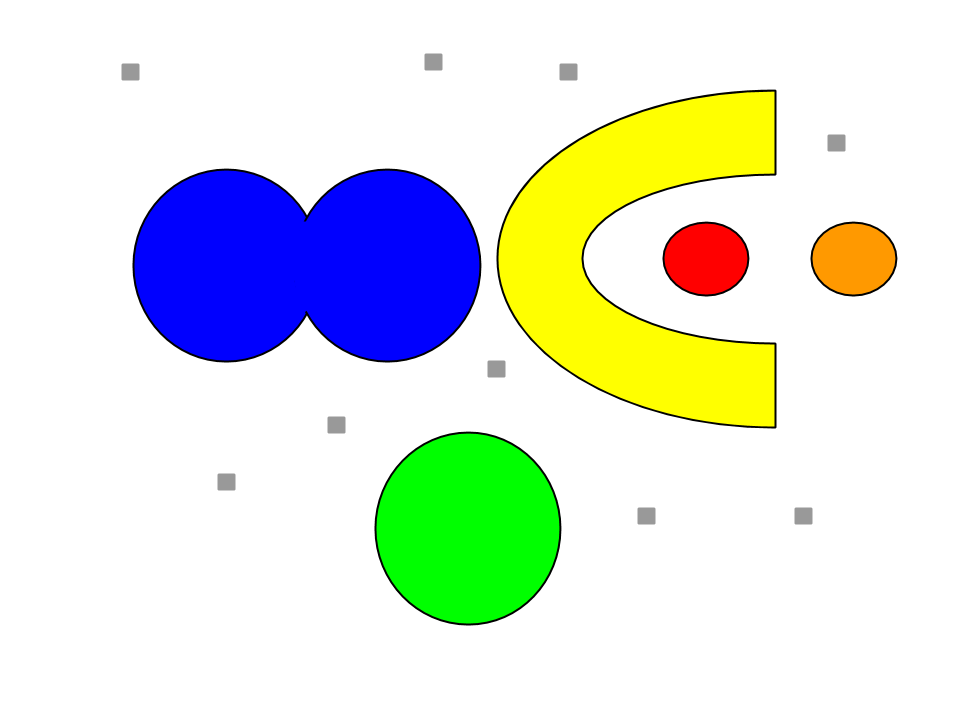
\includegraphics[width=.5\linewidth]{img/densityClusters.png}
  \caption{Density-Based Clusters (Gray squares represent noise)}
  \label{fig:densityClusters}
\end{subfigure}%
\vspace*{0.5cm} 
\begin{subfigure}{.5\textwidth}
  \centering
  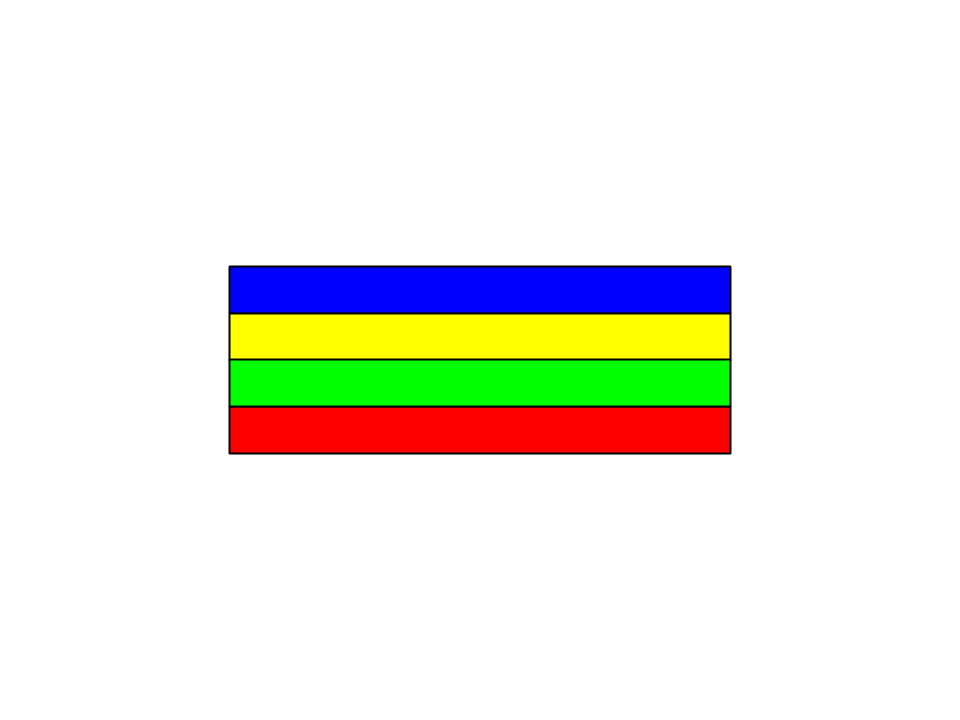
\includegraphics[width=.5\linewidth]{img/conceptualClusters.png}
  \caption{Conceptual Clusters (Points in cluster have y-coordinate from specific range, omitting x-coordinate)}
  \label{fig:conceptualClusters}
\end{subfigure}%
\begin{subfigure}{.5\textwidth}
  \centering
  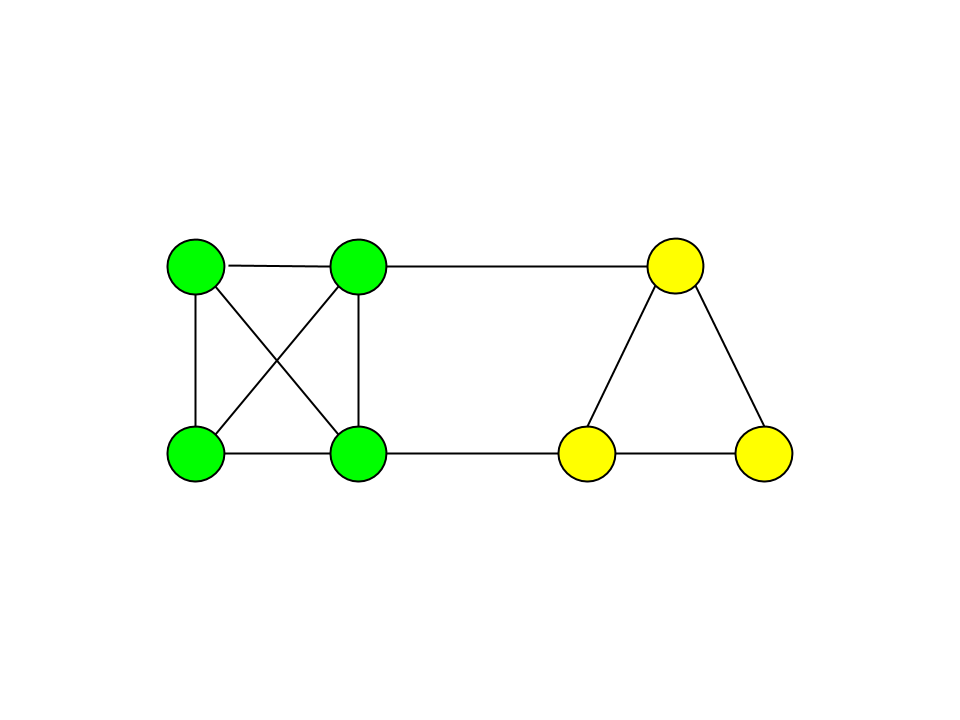
\includegraphics[width=.5\linewidth]{img/graphClusters.png}
  \caption{Graph-Based Clusters}
  \label{fig:graphClusters}
\end{subfigure}%
\caption{Typical cluster models}
\end{figure}

We can also divide clustering algorithms by relationship type:

\begin{description}
\item[Strict partitioning clustering] Objects belongs exactly into one cluster
\item[Strict partitioning clustering with outliers] Same as \textit{\textbf{strict partitioning clustering}} but object can be also unassigned. 
\item[Overlapping clustering] Object may belong to multiple clusters and we can specify, how much object belong to each cluster for example in percent.
\item[Hierarchical clustering] Object belongs also into parent clusters.
\end{description}

\section{Clustering Algorithms} \label{sec:clusteringAlgorithms}
 
\section{GPU parallelization}
\subsection{Compute Unified Device Architecture (CUDA)}